\documentclass{article}
\usepackage{graphicx} 
\usepackage{kotex}
\usepackage{listings}
\usepackage{float}

\usepackage[utf8]{inputenc}
\usepackage{listings}
\usepackage{xcolor}

\lstset{
  basicstyle=\ttfamily\small,
  keywordstyle=\color{blue},
  commentstyle=\color{gray},
  stringstyle=\color{red},
  showstringspaces=false,
  columns=fullflexible,
  keepspaces=true,
  language=Lisp,
  morecomment=[l]{;}
}



\title{프로그래밍 언어 HW4 제출}
\author{C335186 서장훈}
\date{27, May, 2025}

\begin{document}

\maketitle


\section{LISP에 관해 공부한 내용, 느낀점}
Lisp는 포트란에 이어 가장 오래된 고급 언어 중 하나이다. LISP의 큰 특징 중 하나는 코드가 리스트 형태로 작성된다는 것이다. 코드를 작성하면서 익숙한듯하면서도 낯선 구조때문에 첫 함수를 정의할 때까지 굉장히 오랜 시간이 걸렸다. 하지만 문법적으로 매우 단순한 구조를 가지고 있어서 감을 잡고 난 뒤에는 비교적 편하게 했다. \\ \\ 연산을 할 때에도 (+ 1 2)와 같이 전위 표기법을 이용한다. 첫번째 요소를 함수나 연산자를 쓰고, 뒤로는 인자를 써준다. 수학적 표현과 다르지만 기계 처리에는 용이하다고 한다. \\ \\
Lisp는 함수형 프로그래밍 언어로도 대표격으로 여겨진다. 함수를 변수에 할당하거나 인자로 넘기는 구조가 특히 hw4a.lisp에 많이 나오는데 이러한 특성은 고차 함수의 구현을 자연스럽게 만들어준다. 그리고 hw4a에서는 반복문을 재귀를 사용해서 표현했다. 코드를 짜보면서 Lisp의 구조를 더 잘 느껴볼 수 있었다. \\ \\
Lisp를 구성하는 기본 단위는 atom, list, string 이다. 리스트는 또한 중첩이 가능하다. 코드 대부분은 괄호로 감싸진 리스트 구조로 이루어져있고, 중첩이 많아지고 괄호의 개수가 많이질수록 깊이가 깊어지는것이 특징이다. \\ \\
데이터를 다루기 위한 리스트 연산 함수로는 car, cdr, cons가 있다. car는 리스트의 첫요소를 반환하고, cdr은 첫 요소를 제외한 나머지를 리스트로 반환하고, cons는 새로운 요소를 리스트의 앞에 덧붙여 새로운 리스트를 생성한다. 이외에도 nth 같은 여러 내장 함수들이 존재한다. \\ \\
함수 정의는 defun으로 정의하며, 아래 코드들은 전부 함수들로 정의해서 문제를 풀어나갔다. setq를 통해 변수의 정의를 해줄 수 있고, quote 나 ' 연산자를 사용하여 리스트 전체를 값으로 저장할 수도 있다. 출력은 print, princ, pin1 등이 있고 print는 ""를 포함한 내용을 출력하고 개행 문자는 무시하고 한줄의 공백과 한칸의 공백을 생성한다. prin1은 ""을 포함한 내용을 출력하고 개행문자를 무시한다. princ는 ""를 무시한 내용을 출력하고 나머지는 prin1과 동일하다. 또한 줄바꿈을 하고 싶을때 terpri를 사용해주었다. \\ \\
이러한 기초 문법들을 바탕으로 hw4a, hw4b 문제를 풀어보았으며 Lisp의 기본 문법과 리스트연산, 함수 정의, 전위 표기법 등을 익혔고 Lisp에 대한 전반적인 이해도도 함께 키울 수 있었다.

\section{hw4a.lisp}
\subsection{hw4a.lisp 코드(주석포함)}
\begin{lstlisting}

;; Function to receive input n

; Prompts the user to enter the value of n
(defun set-n ()
    (princ "input your N. n = ")
    (read))

;; ----------


;; Functions to construct the board

; Creates a single row (list of 0s)
; Used to build the board (chessboard)
(defun make-row (n)
    (if (= n 0)
        '()
        (cons 0 (make-row (- n 1)))))

; Constructs a 2D board using make-row above
; Creates m rows of size n, forming an n*n board
(defun set-help (m n)
	(if (= m 0)
		'()
		(cons (make-row n) (set-help (- m 1) n))))

; Final function to build the board
(defun set-board (n)
	(set-help n n))

;; ----------



;; Backtracking algorithm will be used to solve the problem
;; It explores all rows, checks if placement is valid, places a queen, 
; - and proceeds to the next column. If blocked, it backtracks.



;; Function to try placing a queen in each column recursively

; Attempts to find a valid position for a queen in each column starting 
; - from col = 0
(defun solve (board col n)
	(if (= col n)
		'()
		(solve-row board 0 col n)))

; Tries all rows in the current column. Stops when row = n.
; Uses is-safe to check whether a queen can be placed at (row, col)
; Recursive form of a loop
(defun solve-row (board row col n)
	(if (= row n)
		'()
		(if (is-safe board row col n)
			(solve-row-safe board row col n)
			(solve-row board (+ row 1) col n))))


; replace-in-board is used to place a queen at a specific location
; If is-safe returns true, proceeds here
; Places a queen (1) at the position and creates a new board
; If at the last column (col = n-1), calls add-solution to save the board
; Otherwise, proceeds to next column
(defun solve-row-safe (board row col n)
	(setq board-with-queen (replace-in-board board row col 1))
	(if (= col (- n 1))
		(add-solution board-with-queen n)
		(solve board-with-queen (+ col 1) n))
	(solve-row board (+ row 1) col n))



; As mentioned above, to indicate that a queen has been placed at a 
; -specific position on the board,
; we need to update the board state.
; This function was created for that purpose.
; It creates a new list by changing the value at the given 
; -column (col) in the given row.
; If col is 0, it replaces the first value and appends the 
; -rest of the row as is.
(defun replace-in-row (row col val)
	(if (= col 0)
		(cons val (cdr row))
		(cons (car row) (replace-in-row 
        (cdr row) (- col 1) val))))


; When row is 0, only that row is modified (others remain unchanged).
; Calls replace-in-row to update the specific row.
(defun replace-in-board (board row col val)
	(if (= row 0)
		(cons (replace-in-row (car board) col val) (cdr board))
		(cons (car board) (replace-in-board (cdr board) 
            (- row 1) col val))))

; ----------




; From here on are the helper functions for is-safe.
; They check if there's a queen in any direction a queen can move 
; -(only the left side is checked).
; Only the left side is checked because the algorithm places 
; -queens from left to right, 
; so no queens exist on the right yet.
; If any position has a 1 (indicating a queen), it returns nil
; otherwise, it returns t for safe.
(defun is-safe (board row col n)
	(if (check-left board row col)
		(if (check-up-left board (- row 1) (- col 1))
			(check-down-left board (+ row 1) (- col 1) n)
			nil)
		nil))

; Checks if there is a queen to the left.
; The helper function used here will be explained below.
(defun check-left (board row col)
	(if (= col 0)
		t
		(if (= (get-value board row (- col 1)) 1)
			nil
			(check-left board row (- col 1)))))

; Checks the upper-left diagonal.
; The helper function used here will be explained below.
(defun check-up-left (board row col)
	(if (or (< row 0) (< col 0))
		t
		(if (= (get-value board row col) 1)
			nil
			(check-up-left board (- row 1) (- col 1)))))

; Checks the lower-left diagonal.
; The helper function used here will be explained below.
(defun check-down-left (board row col n)
	(if (or (>= row n) (< col 0))
		t
		(if (= (get-value board row col) 1)
			nil
			(check-down-left board (+ row 1) (- col 1) n))))


; Retrieves the value at (row, col) from the board.
; Uses nth to access the elements.
(defun get-value (board row col)
	(nth col (nth row board)))

; -----------


;; From here, functions for result output


; Extracts the coordinates of queens from each row of the board.
(defun extract-positions (board row n)
	(if (= row n)
		'()
		(cons (find-queen-in-row (nth row board) 0 (+ row 1))
		      (extract-positions board (+ row 1) n))))

; Finds the column in a row where a queen (1) is located.
(defun find-queen-in-row (row col row-num)
	(if (null row)
		(list row-num 0)
		(if (= (car row) 1)
			(list row-num (+ col 1))
			(find-queen-in-row (cdr row) 
            (+ col 1) row-num))))


; Adds a solution (board with queens).
; Although the board is represented as a list of 0s and 1s,
; extract-positions is used here to prepare it for output.
(defun add-solution (board n)
	(print (extract-positions board 0 n)))

; ----------

; Get input n and print the result
(setq n (set-n))
(setq board (set-board n))
(setq solutions (solve board 0 n))


; If n is 2 or 3, there are no solutions 
;handle this case separately.
(if (or (= n 2) (= n 3))
	(print nil))


\end{lstlisting}

\newpage







\subsection{hw4a.lisp 작동 방식}
이 코드는 백트래킹 방식을 기반으로 만들어진 구조이다. set-n 함수를 통해 체스판의 크기인 N을 입력한다. 이 값은 N * N 보드를 set-board 함수를 통해 구성한다. 보드에 퀸을 놓은 자리는 1로 표현하고, 그렇지 않으면 0으로 표시한다. \\ 

이후 solve 함수를 통해 본격적으로 퀸 배치를 해본다. solve 함수는 열(col)을 기준으로 한 칸씩 전직하며 각 열마다 가능한 행들을 탐색한다. 이때 solve-row 함수가 호출되어 현재 열의 각 행에 퀸을 놓을 수 있는지 판단하고, 가능하다면 해당 위치에 퀸을 놓고 다음 열로 재귀적으로 넘어간다. 퀸을 배치할 수 있는가에 대해서는 is-safe 함수를 사용한다. 이 함수는 현재 위치 기준으로 왼쪽, 왼쪽 아래 위 대각선 방향을 검사하여 퀸의 존재 여부를 파악한다. 퀸이 존재하면 nil을 그렇지 않다면 t를 반환한다. \\

만약 퀸을 놓을 수 있다면 solve-row-safe 이동하여 퀸을 배치해준다. 이때 replace-in-board 와 replace-in-row 함수를 사용하여 새 보드를 생성한다. 직접 하나만 수정하는 것이 아니다. \\
마지막 열인 n-1에 도달하게 된다면 해당 보드가 하나의 해가 되므로 add-solution 함수가 호출된다.\\ \\ 

add-solution 함수는 보드에서의 퀸 위치를 좌표를 추출하기 위해 extract-positions 함수를 호출한다. 이 함수는 각 행을 확인해서 1이 존재하는 열을 (row col) 형식의 리스트로 변환한다. 이렇게 얻은 결과가 화면에 출력되게 된다. \\ \\

재귀 호출이 끝났다면 solve-row 함수로 돌아와서 다음 행을 탐색하게 되며 이 과정을 반복하여 가능한 모든 퀸 배치를 찾게 된다. 이처럼 퀸을 두고 다음 열을 나아갔다가 다시 돌아오고 탐색하는 등의 방식은 백트래킹 알고리즘 구조로 볼 수 있기 때문에 백트래킹 기반의 구조가 말한것이다. \\ \\

마지막으로, 2와 3을 입력받는 해가 존재하지 않는 특이한 상황의 경우에는 예외적인 케이스이므로 nil을 출력하도록 별도 처리해주었다. \\
여기까지가 hw4a.lisp의 동작 방식에 대한 설명이다.

\newpage

\subsection{hw4a.lisp 실행 결과}

문제에서 요구하는 N=4 인 경우이다. \\

\begin{figure}[H]
    \centering
    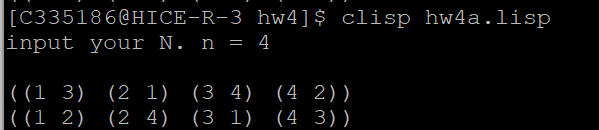
\includegraphics[width=1\linewidth]{hw4a_result.png}
    \caption{hw4a.lisp 결과}
    \label{fig:enter-label}
\end{figure}

\newpage


추가로 N=4 이외에 다른 경우일 때에도 찾아보았다. 

\begin{figure}[H]
    \centering
    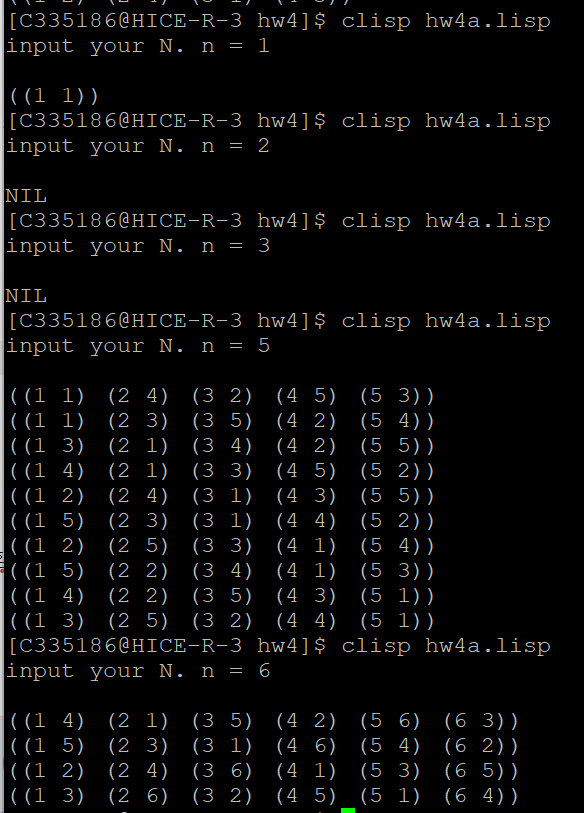
\includegraphics[width=1\linewidth]{hw4a_result_plus.png}
    \caption{hw4a.lisp 결과 - 추가}
    \label{fig:enter-label}
\end{figure}

\newpage



\section{hw4b.lisp}
\subsection{hw4b.lisp 코드(정렬과정 포함O, 주석포함)}
\begin{lstlisting}

(defun insertion-sort (arr)
  ; Store the length of the array in n
  (let ((n (length arr)))
  
    ; Loop from index i = 1 to n - 1 (outer loop of insertion sort)
    (loop for i from 1 below n do
      ; key is the current value to insert, taken from arr[i]
      (let ((key (nth i arr))
            ; j is the index of the last sorted element to the left of key
            (j (- i 1)))
        
        ; Shift elements greater than key one position to the right
        ; Continue while j >= 0 and arr[j] > key
        (loop while (and (>= j 0) (< key (nth j arr))) do
          ; Copy arr[j] to arr[j + 1] (shift right by one position)
          (setf (nth (+ j 1) arr) (nth j arr))
          ; Decrement j to move left
          (decf j))

        ; After shifting, insert key at the correct position (j + 1)
        (setf (nth (+ j 1) arr) key))
      
      ; Print the array after each insertion step to observe the sorting progress
      (print arr))

    ; Return the sorted array
    arr))

; Test cases
(setq tc1 '(83 72 65 54 47 33 29 11))
(setq tc2 '(11 33 23 45 13 25 8 135))

; Sort and print the progress for each test case
(insertion-sort tc1)
(terpri) ; Print a newline
(insertion-sort tc2)


\end{lstlisting}
\newpage


\subsection{hw4b.lisp 작동 방식}

위 Insertion Sort 코드는 우선 list의 arr을 인자로 받는다. \\
내부적으로는 먼저 리스트의 길이를 계산해서 변수 n에 저장한다. 외부 반복문의 범위를 결정하기 위해서 사용되는 값이다. tc 의 경우에선, 리스트 길이가 8이므로  인덱스 1부터 7까지를 차례로 검토하는 것이다. 인덱스 0의 경우에는 비교기준이 되는 초기 정렬 구간으로 사용된다. \\ \\

외부에서는 i 인덱스를 1부터 n 보다 작을 때까지 반복시킨다. 이 i번째 요소가 현재 정렬 대상이 되며 다르게 말하자면 삽입하려는 요소인 셈이다. 이 요소를 리시트에서 꺼낸 뒤 key 변수에 따로 저장해둔다. (요소 이동 시 현재 요소에 문제가 생기지 않기 하기 위해) \\ \\

그러고 난 뒤 key를 정렬된 부분(인덱스 0 ~ i-1) 이랑 비교하면서 key보다 큰 값들을 한칸씩 오른쪽으로 이동시킨다. 이때 비교는 j 인덱스를 이용한다. j는 처음에는 i-1로 시작하고 리스트 앞쪽으로 한칸씩 이동하면서 key보다 큰 값을 찾는다. 비교조건은 j가 0 이상인지, arr[j]가 key보다 큰지이다. 이 조건이 참이라면 arr[j] 값을 arr[j+1]로 복사한다. (더 큰값을 오른쪽으로 밀어내기) 이러한 과정을 통해 key가 들어갈 적절한 자리를 비워낸다. j는 그 다음 왼쪽 요소를 비교하기 위해 1씩 감소시킨다. 이걸 현재 정렬된 구간의 가장 왼쪽까지 진행하고, key보다 작거나 같은 값을 만나면 멈춘다. \\ \\

내부 반복이 만약 멈췄다면 j는 key가 삽입돼야할 위치보다 한칸 앞을 가리키게된다. 따라서 key는 j+1위치에 삽입되는 것이다. 이떄 setf를 통해 arr[j+1] 자리에 key를 넣는다. 이렇게 리스트의 앞쪽을 i번째까지 오름차순으로 정렬시킨것이다. \\ \\

이걸 외부 반복이 끝날때까지 print 함수를 호출하면서 리스트의 상태를 출력한다면? 문제의 추가조건인 정렬되는 과정을 보이는 것까지 전부 만족시킬 수 있다. \\ \\




\newpage
\subsection{hw4b.lisp 실행 결과}

\begin{figure}[H]
    \centering
    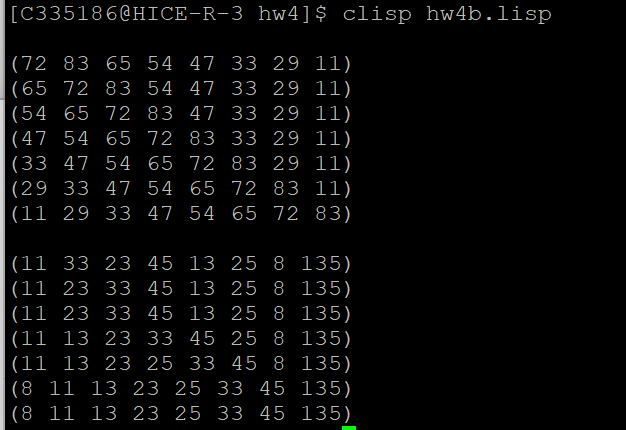
\includegraphics[width=1\linewidth]{hw4b_result.png}
    \caption{hw4b.lisp 실행결과}
    \label{fig:enter-label}
\end{figure}
\end{document}

